%
% The first command in your LaTeX source must be the \documentclass command.
\documentclass[sigconf]{acmart}

%
% defining the \BibTeX command - from Oren Patashnik's original BibTeX documentation.
\def\BibTeX{{\rm B\kern-.05em{\sc i\kern-.025em b}\kern-.08emT\kern-.1667em\lower.7ex\hbox{E}\kern-.125emX}}
    
% Rights management information. 
% This information is sent to you when you complete the rights form.
% These commands have SAMPLE values in them; it is your responsibility as an author to replace
% the commands and values with those provided to you when you complete the rights form.
%
% These commands are for a PROCEEDINGS abstract or paper.
\copyrightyear{2018}
\acmYear{2018}
\setcopyright{acmlicensed}
\acmConference[CU Boulder '19]{CU Boulder '19: CSCI 4502 - Data Mining}{Fall, 2019}{Boulder, CO}
\acmBooktitle{CU Boulder '19: CSCI 4502 - Data Mining, Fall, 2019, Boulder, CO}
\acmPrice{0.00}

%
% These commands are for a JOURNAL article.
%\setcopyright{acmcopyright}
%\acmJournal{TOG}
%\acmYear{2018}\acmVolume{37}\acmNumber{4}\acmArticle{111}\acmMonth{8}
%\acmDOI{10.1145/1122445.1122456}

%
% Submission ID. 
% Use this when submitting an article to a sponsored event. You'll receive a unique submission ID from the organizers
% of the event, and this ID should be used as the parameter to this command.
%\acmSubmissionID{123-A56-BU3}

%
% The majority of ACM publications use numbered citations and references. If you are preparing content for an event
% sponsored by ACM SIGGRAPH, you must use the "author year" style of citations and references. Uncommenting
% the next command will enable that style.
%\citestyle{acmauthoryear}

%
% end of the preamble, start of the body of the document source.
\begin{document}

%
% The "title" command has an optional parameter, allowing the author to define a "short title" to be used in page headers.
\title{World of Warcraft Classic: Auction House Strategy Analysis}

%
% The "author" command and its associated commands are used to define the authors and their affiliations.
% Of note is the shared affiliation of the first two authors, and the "authornote" and "authornotemark" commands
% used to denote shared contribution to the research.
\author{Nikolai Alexander}
\affiliation{%
\department{CSCI 4502}
  \institution{University of Colorado, Boulder}
  \city{Boulder}
  \state{CO}
  \country{USA}}
\email{nial3328@colorado.edu}

%
% By default, the full list of authors will be used in the page headers. Often, this list is too long, and will overlap
% other information printed in the page headers. This command allows the author to define a more concise list
% of authors' names for this purpose.
\renewcommand{\shortauthors}{Alexander}

%
% The abstract is a short summary of the work to be presented in the article.
\begin{abstract}
I am going to be comparing different investment strategies in the World of Warcraft Classic Auction House to determine which strategy performs the best. The four strategies I am planning on using are optimizing unit profit based on minimizing cost and maximizing revenue, minimizing turnaround time for unit investments, buying and selling based on relevance to game content, and buying and selling based off weekly price trends. The strategies are going to be implemented using a different character for each strategy. The evaluation is going to be through comparing the net gain of each of the 4 characters at the end of a set period with the conclusion that the best performing strategy is the most effective.
\end{abstract}

%
% The code below is generated by the tool at http://dl.acm.org/ccs.cfm.
% Please copy and paste the code instead of the example below.
%
\begin{CCSXML}
<ccs2012>
<concept>
<concept_id>10002950.10003648.10003704</concept_id>
<concept_desc>Mathematics of computing~Multivariate statistics</concept_desc>
<concept_significance>500</concept_significance>
</concept>
<concept>
<concept_id>10002951.10002952.10002953.10002955</concept_id>
<concept_desc>Information systems~Relational database model</concept_desc>
<concept_significance>300</concept_significance>
</concept>
</ccs2012>
\end{CCSXML}

\ccsdesc[500]{Mathematics of computing~Multivariate statistics}
\ccsdesc[300]{Information systems~Relational database model}

%
% Keywords. The author(s) should pick words that accurately describe the work being
% presented. Separate the keywords with commas.
\keywords{Video Game Economy Analysis, Economic Trend Prediction, World of Warcraft Classic, Auction House}

%
% This command processes the author and affiliation and title information and builds
% the first part of the formatted document.
\maketitle

\section{Introduction}
World of Warcraft Classic (WoW Classic) is a remake of the original Massive Multiplayer Online Role-Playing Game (MMORPG), World of Warcraft, released on November 23, 2004. Within this game, players can complete quests, explore dungeons, and trade with non-player characters (NPCs) and other players. One of the major aspects of WoW classic is its complex economy, specifically its auction house. The auction house is a trading hub that allows players to buy and sell items with each other for a price set by the seller. Pricing is competitive and volatile, with players continuously undercutting and buying out each other in an attempt to control the market. Prices can be affected by many factors, such as popularity of the item, relevance to current content, and popular weekly routines of the player-base. Price fluctuations also have an element on randomness to them due to the freedom of the market.

One example we can look at is the \href{https://classic.wowhead.com/item=13457/greater-fire-protection-potion}{Greater Fire Protection Potion}. The most popular content played in the game is raiding. Raiding is when a group of 25 to 40 players attempt to complete a very difficult instance, usually ending in defeating a major antagonist. In the current phase of WoW Classic, the two raids are The Molten Core and Onyxia’s Lair. Both instances are focused around mitigating fire damage, with the final bosses being Ragnaros the Firelord and Onxia, the daughter of the dragon Deathwing. Because of this, the most popular item bought for this content is Greater Fire Protection Potions. However, due to the large amount of organization required to set up a raid group, majority of raid groups set schedules raid times – usually around the weekly instance reset which is Tuesday. Thus, the price of Greater Fire Protection Potions rise to 10 to 15 gold on Tuesdays and Wednesdays and begin to drop down to as low as 3 to 5 gold by the end of the week.

I am going to be analyzing price trends of a few different items, such as the Greater Fire Protection Potion and \href{https://classic.wowhead.com/item=7068/elemental-fire}{Elemental Fire} – a common crafting item used for producing powerful items, including Greater Fire Protection Potions. I am going to look for correlations with other item prices, player population statistics such as popular classes and gear, and scheduled content within the game. I am also going to analyze how minimizing purchasing costs and maximizing revenue compares minimizing item turnaround time.

Just like real work stock market indexes, such as the S\&P500, there are myriad, potential strategies one could come up to exploit the behavior the auction house. Trying to keep track of prices for all 15914 items in existence in the game is not possible and will almost always perform poorly. I am going to be analyzing four strategies – Predicting the weekly trends of a few items, analyzing weekly content updates and buying and selling items that reflect those updates, optimizing unit profit for items by predicting minimum cost and maximum revenue, and finally, optimizing unit turnaround time by buying and selling items with high sales rates and high volatility.

The challenges I foresee lie in collecting the data and finding a control group to mitigate any bias for any one strategy. Unfortunately, Blizzard does not have an API for WoW Classic, so I need to collect my own data using file parsing and web scraping - I will also need to find a way to store the data, whether locally or on a server. Some control groups I am looking into are controlling for price range in which I buy and sell the items. However, this will be difficult as certain strategies rely on high unit profit margins while other strategies rely on a high rate of small unit profits. One idea I am considering implementing is tracking 3 to 5 items in different price ranges for each strategy and balance the mean price between all four strategies. I am also planning on controlling for time range; all four strategies are going to start on the same date and end on the same date, which will allow for an easy calculation of the rate of growth.

This analysis will not only have applied functionality, but will also give some great insights into how an in-game economy works. This can be further used to see parallels between a virtual economy and the real-world economy. It will also give insight into what factors play the biggest part in the behavior of the economy. How much does game-content actually affect prices? How much of the economy is predictable, and how much is random?


\section{Related Work}
	Complex analysis on MMORPG economies has been down before and even is the center of the gameplay for games such as \href{https://www.eveonline.com/article/prg4uv/monthly-economic-report-april-2019}{Eve Online}, but as for formal economic research on World of Warcraft Classic’s economy, none has been done so far. However, there have been many different tools for analyzing the World of Warcraft economy built by the WoW Community, such as the in-game modifications \href{https://www.curseforge.com/wow/addons/auctioneer}{Auctioneer} and \href{https://www.tradeskillmaster.com/}{TradeSkillMaster}, the subreddit \href{https://www.reddit.com/r/woweconomy/}{Wow Economy}, and the online economic reporting website \href{https://www.reddit.com/r/woweconomy/}{Booty Bay Gazette}.

Where my approach differs from these tools/methods is none of these keep historical data or try to predict future prices. I am going to be storing all scanned data in a postgres database using \href{http://aws.amazon.com/}{Amazon Web Services}, and will have access to all data starting from the first scan. Using this method, I will be able to efficiently isolate specific items, time frames, and price ranges to separate sub-data sets, all while still maintaining access to all of the data I may need. I  will be able to use the power of postgresql and the AWS server computing power to pre-process the data, which will free up computing power and local resources for analysis. I will also be able to store a much larger amount of data than if I were to keep it in csv format. I can store data on game statistics, player population data, future content information, as well as item statistics for every item in the game. This will widely increase the freedom for finding the best method of price prediction.

My approach also differs from the above tools, as none of these use a particular strategy in viewing the economy. They are purely reporting tools to be interpreted by the end user. My work is using specific strategies in order to exploit the market for profit gain. I am going to be looking at four different strategies to see which one performs the best against the auction house economy.

\section{Proposed Work}
The data collection is going to a large portion of the work for the project. While Blizzard has a public API for the current World of Warcraft, they announced that they would refrain from publicizing one for classic, with the motive of staying true to the original 2004 release. This means I will need to get creative in my data collection methods. I am going to collect data on game-content, and player statistics by web-scraping the \href{https://classic.wowhead.com/}{Classic WoWHead} website, the largest public World of Warcraft database. I also do a lot of manual research by reading patch releases, studying raid mechanics, and posting/searching for public surveys from the WoW Classic community.

I will need to produce my own auction house data, as there is currently none publicly available. I will use the Blizzard endorsed modification, TradeSkillMaster, to scan the auction house. After each scan, TradeSkillMaster stores the data in a LUA file called AppData.lua in the game files, which can then be parsed and stored in a data frame. While creating a script that automatically logs into the game and scans the data on a schedule is against \href{https://www.blizzard.com/en-us/legal/fba4d00f-c7e4-4883-b8b9-1b4500a402ea/blizzard-end-user-license-agreement}{Blizzard’s End User License Agreement} under botting, TradeSkillMaster has the advantage of an external app that updates whenever any player using the mod scans the auction house. Thus, I can passively collect auction house data without breaking any rules. I have a written a script that parses the data, cleans it, and inserts it into a public AWS Postgresql Database every time the AppData.lua file updates with new data. In order passively scan and store up-to-date data, I have the script running on a server created from an old computer.

My next task is going to be finding correlations between items, such as which items are used to craft other important items and which items are required to complete the current content. This is going to use a combination of exploratory analysis and independent research through articles and game-guides. I am also going to track price fluctuations, average price ranges, and outliers using histograms and bar-charts. I am hypothesizing that prices for the most part follow a Gaussian distribution, which should make it easier to keep track of trends.

The next thing I am planning on analyzing, is how prices are affected on a weekly basis. World of Warcraft usually runs on a weekly cycle, due to weekly resets and in-game world events. Thus, my hypothesis for this is prices follow some sort of weekly trend. I am planning on waiting a month before doing this type of analysis, as it  will become more accurate and consistent as my dataset becomes larger.

Even though there is a lot of moving parts to this project, I have a high confidence of being able to complete this by myself. Automating the data collection process frees my time up to focus on the analysis, and I can produce postgresql scripts to automate the pre-processing for me. As of right now, I am planning to avoid using machine learning as I am unclear if breaks Blizzard’s EULA, which means the bulk of my work is going to be dedicated exploratory analysis – such as finding correlations and analyzing trends.

\section{Evaluations}
My main source for evaluating my strategies is going to be comparing the one-month performance between all 4 strategies strategy. I am going to compare how investing with a focus weekly trends compares to focusing on item correlations, and how minimizing cost and maximizing revenue compares to minimizing item turnaround time. My evaluation metric is going to be the final cumulative gains for each of my strategies – whichever strategy ends with the most gold is the most effective. I am going to keep track of this by running each strategy individually with a different character. I am going to start each character with the same exact starting wealth (somewhere between 3-5 gold) to avoid any bias or advantage for any one strategy. Luckily, TradeSkillMaster has built-in functionality to keep track of my revenue/cost/profit over time for up to a year, which means I will not need to be responsible for managing my portfolio’s data.

\begin{figure}[h]
  \centering
  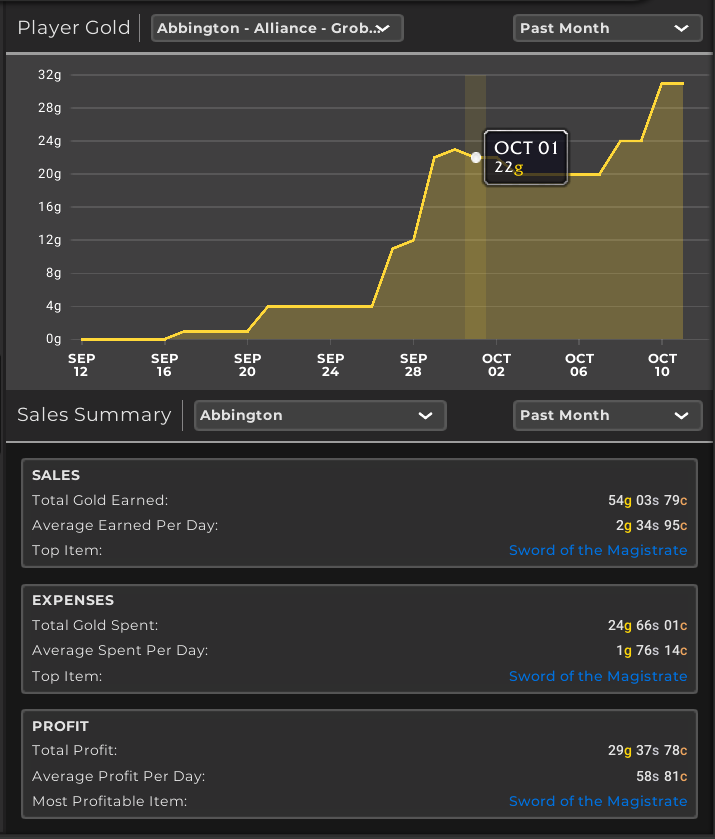
\includegraphics[width=\linewidth]{TSM_Stats}
  \caption{TradSkillMaster Portfolio Summary, screenshotted from inside World of Warcraft Classic.}
  \Description{TradeSkillMaster Portfolio Summary.}
\end{figure}

\section{Milestones}
\begin{enumerate}
	\item Have data mining server up and running $\rightarrow$ October 15
	\item Research most cost-effective items to track, items relevant to content, player population statistics for my server $\rightarrow$ October 25
	\item Mine WoWHead Database of all item data $\rightarrow$ November 1
	\item Begin implementing strategies in game (Create character for each strategy) $\rightarrow$ November 1
	\item Begin exploratory analysis on correlations $\rightarrow$ November 1
	\item Begin weekly trend analysis $\rightarrow$ November 15
	\item End implementing strategies and compare gains between characters $\rightarrow$ December 6
\end{enumerate}

\section{Acknowledgments}
I would like to thank Blizzard Entertainment for allowing me to collect data off of World of Warcraft Classic in order to perform this project. I would also like to thank WoWHead for providing me with all of the data and information I need to effectively produce this project. Apart from the game, I would like to thank Doug Alexander for advising me on teaching me about different investment strategies and helping me formulate the strategies I am going to use for this project.

\section{Honor Code Pledge}
On my honor, as a University of Colorado Boulder student, I have neither given nor received unauthorized assistance. The University of Colorado Honor Code works by receiving the support and participation of all members in the university community. Such an organization is intended to promote a campus culture that consciously upholds the tenets of academic integrity, and moral and ethical conduct.

\section{Citations and Bibliographies}
\begin{enumerate}
	\item Blizzard Entertainment. “Blizzard End User License Agreement.” Blizzard Legal, Blizzard Entertainment, 1 June 2018, www.blizzard.com/en-us/legal/fba4d00f-c7e4-4883-b8b9-1b4500a402ea/blizzard-end-user-license-agreement.
	\item Erorus. “Booty Bay Gazette.” Booty Bay Gazette, The Undermine Journal, 9 Oct. 2019, www.bootybaygazette.com/.
	\item Fanbyte. “World of Warcraft.” Wowhead, 2019, classic.wowhead.com/.
	\item Larrikin, CPP. “Monthly Economic Report - April 2019.” EVE Online, CPP, 13 May 2019, www.eveonline.com/article/prg4uv/monthly-economic-report-april-2019.
	\item “r/Woweconomy.” Reddit, www.reddit.com/r/woweconomy/.
	\item TradeSkillMaster. “Most Advanced Addon for Making Gold in World of Warcraft.” TradeSkillMaster, TradeSkillMaster, 2019, www.tradeskillmaster.com/.
\end{enumerate}

\end{document}
